% Presentation mode: overlays/animations build step-by-step (one page per step).
% For a FLAT distribution PDF (one page per frame, no builds), add 'handout':
%   \documentclass[handout,aspectratio=169,10pt]{beamer}
\documentclass[aspectratio=169,10pt]{beamer}

\usepackage[T1]{fontenc}
\usepackage[utf8]{inputenc}
\usepackage{lmodern}
\usepackage{array}
\usepackage{booktabs}
\usepackage{colortbl}
\usepackage{graphicx}
\graphicspath{{../slides/}}
\usepackage{tikz}
\usetikzlibrary{arrows.meta,positioning,shapes.geometric,fit}

% Auto-generated by slides/generate_slide_assets.py
\newcommand{\CurrentAtlasStatus}{validated}
\newcommand{\CurrentAtlasPolicy}{fixed-policy}
\newcommand{\CurrentAtlasRuns}{30}
\newcommand{\CurrentAtlasEstimators}{17}
\newcommand{\CanonicalEstimatorCount}{17}
\newcommand{\ReadinessIssueCount}{0}

\newcommand{\DynamicTopTable}{%
\begin{tabular}{llrrrr}
\toprule
Estimator & Family & Geo. RMSE & Worst & CPU us & Latency ms \\
\midrule
ESPRIT & Window-based & 0.035 & 0.355 & 89 & 8.3 \\
Koopman (RK-DPMU) & Data-driven & 0.04 & 0.432 & 156 & 12.5 \\
TFT & Window-based & 0.054 & 2.952 & 9 & 16.6 \\
IPDFT & Window-based & 0.054 & 0.59 & 9 & 33.3 \\
SOGI-FLL & Loop-based & 0.063 & 0.844 & 8 & 0 \\
ZCD & Loop-based & 0.063 & 0.65 & 5 & 16.7 \\
SOGI-PLL & Loop-based & 0.065 & 0.457 & 9 & 0 \\
\bottomrule
\end{tabular}%
}

\newcommand{\RfeTopTable}{%
\begin{tabular}{llrrrr}
\toprule
Estimator & Family & Geo. RFE & Geo. RMSE & CPU us & Latency ms \\
\midrule
UKF & Model-based & 6.864 & 0.089 & 11 & 0 \\
EKF & Model-based & 7.406 & 0.384 & 9 & 0 \\
TFT & Window-based & 8.842 & 0.054 & 9 & 16.6 \\
SOGI-FLL & Loop-based & 12.017 & 0.063 & 8 & 0 \\
RA-EKF & Model-based & 14.033 & 0.097 & 13 & 0 \\
PI-GRU & Data-driven & 16.293 & 0.07 & 3509 & 9.1 \\
Koopman (RK-DPMU) & Data-driven & 19.046 & 0.04 & 156 & 12.5 \\
\bottomrule
\end{tabular}%
}

\newcommand{\HarmonicsEndpointTable}{%
\begin{tabular}{llrrr}
\toprule
Estimator & Family & 1\% THD & 30\% THD & Ratio 30/1 \\
\midrule
ZCD & Loop-based & 2.69e-04 & 86.37 & 321452 \\
RA-EKF & Model-based & 0.018 & 0.142 & 7.88 \\
TFT & Window-based & 5.03e-03 & 0.151 & 30.00 \\
EKF & Model-based & 1.21e-03 & 2.426 & 2001 \\
SOGI-PLL & Loop-based & 0.030 & 0.226 & 7.46 \\
UKF & Model-based & 3.48e-03 & 2.301 & 661 \\
SOGI-FLL & Loop-based & 0.010 & 0.283 & 28.28 \\
\bottomrule
\end{tabular}%
}

\newcommand{\RegimeDiagnosticTable}{%
\begin{tabular}{lll}
\toprule
Stress & Estimator & Paper-grade pattern \\
\midrule
RoCoF & LKF & 5.5$\times$ worse on down-ramp at $\pm50$ Hz/s \\
RoCoF & TKEO & 3.9$\times$ worse on down-ramp at $\pm50$ Hz/s \\
RoCoF & RLS & 3.1$\times$ worse on down-ramp at $\pm50$ Hz/s \\
RoCoF & EKF/UKF/RA-EKF & approximately sign-symmetric at $\pm50$ Hz/s \\
Magnitude & ZCD & fails deep sag; remains accurate on matching swell \\
Harmonics & ZCD & best at low THD, collapses above $\sim$20\% THD \\
\bottomrule
\end{tabular}%
}


\definecolor{ofbBlue}{HTML}{156082}
\definecolor{ofbRust}{HTML}{E97132}
\definecolor{ofbPlum}{HTML}{6A4C93}
\definecolor{ofbMoss}{HTML}{8A8F2F}
\definecolor{ofbRed}{HTML}{B23A48}
\definecolor{ofbInk}{HTML}{0E2841}
\definecolor{ofbSoft}{HTML}{F3F5F7}
\definecolor{ofbGreen}{HTML}{196B24}
\definecolor{ofbGold}{HTML}{E97132}
\definecolor{ofbViolet}{HTML}{A02B93}
\definecolor{ofbCanvas}{HTML}{FFFFFF}
\definecolor{ofbMuted}{HTML}{5B677A}
\definecolor{ofbLine}{HTML}{D9E1E8}
\definecolor{ofbNavy}{HTML}{0E2841}
\definecolor{sgsmaTeal}{HTML}{12695F}
\definecolor{sgsmaAqua}{HTML}{A8E6DF}
\definecolor{cardFill}{HTML}{F8FAFB}
\definecolor{cardBorder}{HTML}{CBD7DF}
\newcommand{\sgsmaTitleBg}{figures/sgsma_title_bg.png}
\newcommand{\sgsmaDividerBg}{figures/sgsma_divider_bg.png}
\newcommand{\sgsmaContentBg}{figures/sgsma_content_bg.png}

\usetheme{default}
\usecolortheme[named=ofbBlue]{structure}
\setbeamertemplate{navigation symbols}{}
\setbeamercolor{normal text}{fg=ofbInk,bg=ofbCanvas}
\setbeamercolor{title}{fg=white,bg=ofbNavy}
\setbeamercolor{frametitle}{fg=ofbInk,bg=ofbCanvas}
\setbeamercolor{block title}{fg=white,bg=sgsmaTeal}
\setbeamercolor{block body}{fg=ofbInk,bg=cardFill}
\setbeamercolor{footline}{fg=white}
\setbeamerfont{frametitle}{family=\rmfamily,series=\mdseries,size=\fontsize{16.5}{19}\selectfont}
\setbeamerfont{title}{family=\rmfamily,series=\mdseries,size=\Large}
\setbeamerfont{block title}{series=\bfseries,size=\small}
\setbeamersize{text margin left=8mm,text margin right=8mm}
\usebackgroundtemplate{\includegraphics[width=\paperwidth,height=\paperheight]{\sgsmaContentBg}}
\setbeamertemplate{itemize item}{\raisebox{0.15ex}{\scriptsize\textcolor{ofbBlue}{$\bullet$}}}
\setbeamertemplate{itemize subitem}{\raisebox{0.1ex}{\tiny\textcolor{ofbGold}{$\bullet$}}}
\setbeamertemplate{enumerate item}{\textcolor{ofbBlue}{\insertenumlabel.}}
\setbeamertemplate{blocks}[rounded][shadow=false]
\setbeamertemplate{frametitle}{%
  \vspace{0.58cm}
  \hspace{8mm}\begin{minipage}[t]{0.76\paperwidth}
    \raggedright\hyphenpenalty=10000\exhyphenpenalty=10000
    \usebeamerfont{frametitle}\color{ofbInk}\insertframetitle
  \end{minipage}\par
  \vspace{0.05cm}
}
\setbeamertemplate{footline}{%
  \begin{tikzpicture}[remember picture,overlay]
    \node[anchor=south, text=white, font=\tiny] at ([xshift=-0.08\paperwidth,yshift=0.13cm]current page.south) {\insertframenumber/\inserttotalframenumber};
    \node[anchor=south, text=white, font=\tiny\itshape] at ([xshift=0.10\paperwidth,yshift=0.13cm]current page.south) {\insertsection};
  \end{tikzpicture}%
  \vspace*{0.84cm}%
}

\newcommand{\artifact}[1]{%
  \vspace{0.12em}\par\noindent{\tiny\color{ofbMuted}\raggedright Source: \texttt{#1}\par}%
}
\newcommand{\metric}[2]{\textbf{#1}: #2}
\newcommand{\callout}[1]{%
  \vspace{0.25em}\noindent
  \begin{tikzpicture}
    \node[
      draw=cardBorder,
      fill=cardFill,
      rounded corners=2pt,
      line width=0.45pt,
      inner xsep=7pt,
      inner ysep=6pt,
      text width=0.94\linewidth,
      align=left
    ] {\small #1};
    \draw[sgsmaTeal, line width=1.3pt] ([xshift=0.5pt,yshift=-0.5pt]current bounding box.north west) -- ([xshift=0.5pt,yshift=0.5pt]current bounding box.south west);
  \end{tikzpicture}%
  \vspace{0.15em}
}
\newcommand{\tagpill}[2]{%
  \tikz[baseline=(x.base)]\node[inner xsep=5pt,inner ysep=2pt,rounded corners=2pt,fill=#1!12,draw=#1,text=ofbInk,font=\scriptsize\bfseries] (x) {#2};%
}
\newcommand{\statcard}[3]{%
\begin{tikzpicture}
\node[
  draw=cardBorder,
  fill=cardFill,
  rounded corners=2pt,
  line width=0.55pt,
  inner sep=7pt,
  text width=0.86\linewidth,
  minimum height=1.18cm,
  align=left
] {
{\scriptsize\bfseries\color{ofbMuted}#2}\\[0.10em]
{\Large\bfseries\color{#1}#3}
};
\draw[#1, line width=1.5pt] ([xshift=0.5pt,yshift=-0.5pt]current bounding box.north west) -- ([xshift=0.5pt,yshift=0.5pt]current bounding box.south west);
\end{tikzpicture}}
\newcommand{\evidencetag}[2]{%
  \tikz[baseline=(x.base)]\node[
    fill=#1!10,
    draw=#1,
    text=ofbInk,
    line width=0.55pt,
    rounded corners=2pt,
    inner xsep=5pt,
    inner ysep=2.5pt,
    font=\scriptsize\bfseries
  ] (x) {#2};%
}
\newcommand{\resultclaim}[2]{%
  \vspace{0.1em}\noindent
  \begin{tikzpicture}
    \node[
      draw=#1,
      fill=#1!7,
      line width=0.75pt,
      rounded corners=2pt,
      inner xsep=8pt,
      inner ysep=6pt,
      text width=0.93\linewidth,
      align=left
    ] {\large\color{ofbInk}#2};
    \draw[#1, line width=2.0pt] ([xshift=0.6pt,yshift=-0.6pt]current bounding box.north west) -- ([xshift=0.6pt,yshift=0.6pt]current bounding box.south west);
  \end{tikzpicture}%
}
\newcommand{\insightcard}[3]{%
  \begin{tikzpicture}
    \node[
      draw=#1,
      fill=white,
      rounded corners=2pt,
      line width=0.65pt,
      inner xsep=7pt,
      inner ysep=6pt,
      text width=0.90\linewidth,
      align=left
    ] {
      {\scriptsize\bfseries\color{#1}#2}\\[-0.05em]
      {\small #3}
    };
  \end{tikzpicture}%
}
\newcommand{\atlaspreviewbanner}{%
  \vspace{-0.10cm}%
  \noindent
\begin{tikzpicture}
    \node[
      anchor=west,
      rounded corners=2pt,
      fill=ofbRust!12,
      draw=ofbRust,
      line width=0.55pt,
      text=ofbInk,
      font=\scriptsize\bfseries,
      inner xsep=5pt,
      inner ysep=3pt
    ] at (0,0)
    {ATLAS SEVERITY SWEEP: pilot run, $n=1$, default controller policy};
  \end{tikzpicture}\par\vspace{-0.10cm}%
}
\newcommand{\readinessmetricbanner}{%
  \vspace{-0.10cm}%
  \noindent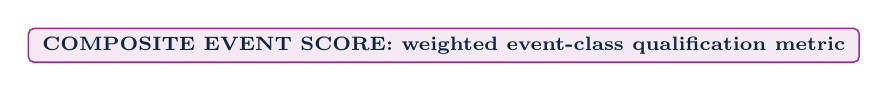
\begin{tikzpicture}
    \node[
      anchor=west,
      rounded corners=2pt,
      fill=ofbViolet!10,
      draw=ofbViolet,
      line width=0.55pt,
      text=ofbInk,
      font=\scriptsize\bfseries,
      inner xsep=5pt,
      inner ysep=3pt
    ] at (0,0)
    {COMPOSITE EVENT SCORE: weighted event-class qualification metric};
  \end{tikzpicture}\par\vspace{-0.10cm}%
}
\newcommand{\extendedresultsbanner}{%
  \vspace{-0.10cm}%
  \noindent
\begin{tikzpicture}
    \node[
      anchor=west,
      rounded corners=2pt,
      fill=ofbBlue!9,
      draw=ofbBlue,
      line width=0.55pt,
      text=ofbInk,
      font=\scriptsize\bfseries,
      inner xsep=5pt,
      inner ysep=3pt
    ] at (0,0)
    {OPENFREQBENCH EXPANSION: 18 estimators, 33 scenarios, $n=5$ seeds per scenario};
  \end{tikzpicture}\par\vspace{-0.10cm}%
}
\newcommand{\diagbanner}{%
  \vspace{-0.10cm}%
  \noindent
\begin{tikzpicture}
    \node[
      anchor=west,
      rounded corners=2pt,
      fill=ofbRust!12,
      draw=ofbRust,
      line width=0.55pt,
      text=ofbInk,
      font=\scriptsize\bfseries,
      inner xsep=5pt,
      inner ysep=3pt
    ] at (0,0)
    {DIAGNOSTIC PILOT: limited-$n$ or subset sweep --- do not read as qualification evidence};
  \end{tikzpicture}\par\vspace{-0.10cm}%
}
\newcommand{\papergradebanner}{%
  \vspace{-0.10cm}%
  \noindent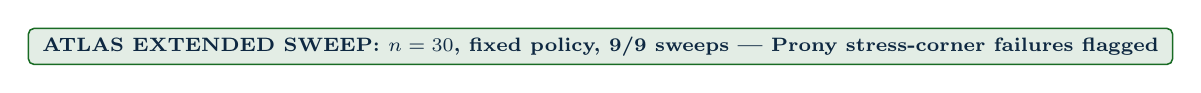
\begin{tikzpicture}
    \node[
      anchor=west,
      rounded corners=2pt,
      fill=ofbGreen!12,
      draw=ofbGreen,
      line width=0.55pt,
      text=ofbInk,
      font=\scriptsize\bfseries,
      inner xsep=5pt,
      inner ysep=3pt
    ] at (0,0)
    {ATLAS EXTENDED SWEEP: $n=30$, fixed policy, 9/9 sweeps --- Prony stress-corner failures flagged};
  \end{tikzpicture}\par\vspace{-0.10cm}%
}
\newcommand{\sectionframe}[3]{%
\begingroup
\usebackgroundtemplate{\includegraphics[width=\paperwidth,height=\paperheight]{\sgsmaDividerBg}}%
\begin{frame}[plain]
\begin{tikzpicture}[remember picture,overlay]
  \node[anchor=center, text=white, align=center, font=\fontsize{27}{32}\selectfont\rmfamily, text width=0.72\paperwidth] at ([yshift=0.25cm]current page.center) {\hyphenpenalty=10000\exhyphenpenalty=10000 #2};
  \node[anchor=center, text=white, align=center, font=\large, text width=0.70\paperwidth] at ([yshift=-0.95cm]current page.center) {\hyphenpenalty=10000\exhyphenpenalty=10000 #3};
\end{tikzpicture}
\end{frame}
\endgroup
}

\title[SGSMA 2026]{Benchmarking Dynamic Frequency Estimators for Low-Inertia IBR Grids}
\subtitle{Latency, trip-risk, and deployability under IBR stress}
\author{Jorge L. Mayorga Taborda, Yessica Africano Rodriguez, Fernando Jimenez}
\institute{Universidad de los Andes}
\date{May 25, 2026}
\newif\ifbackupframes
\backupframesfalse
\newif\iforalcompact
\oralcompacttrue

\begin{document}

{
\setbeamertemplate{footline}{}
\begin{frame}[plain,label=title]
\begin{tikzpicture}[remember picture,overlay]
  \node[anchor=center] at (current page.center) {\includegraphics[width=\paperwidth,height=\paperheight]{\sgsmaTitleBg}};
  \node[anchor=west, text=white, align=left, font=\fontsize{18}{23}\selectfont\rmfamily\itshape, text width=0.72\paperwidth] at ([xshift=0.056\paperwidth,yshift=-0.45cm]current page.west) {
    Benchmarking Dynamic Frequency\\[-0.05em]
    Estimators for Low-Inertia IBR Grids
  };
  \node[anchor=west, text=white, align=left, font=\scriptsize\itshape, text width=0.72\paperwidth] at ([xshift=0.068\paperwidth,yshift=-1.75cm]current page.west) {
    Jorge L. Mayorga Taborda, Yessica Africano Rodriguez, Fernando Jimenez
  };
  \node[anchor=west, text=white, align=left, font=\tiny, text width=0.66\paperwidth] at ([xshift=0.068\paperwidth,yshift=-2.14cm]current page.west) {
    Universidad de los Andes \quad | \quad SGSMA 2026
  };
\end{tikzpicture}
\end{frame}
}

\section{Motivation}
\sectionframe{}{Motivation}{Why frequency estimation in low-inertia IBR grids is hard}

\begin{frame}[label=fieldevents]{Field events define the benchmark stress model}
\vspace{-0.35em}
\begin{center}
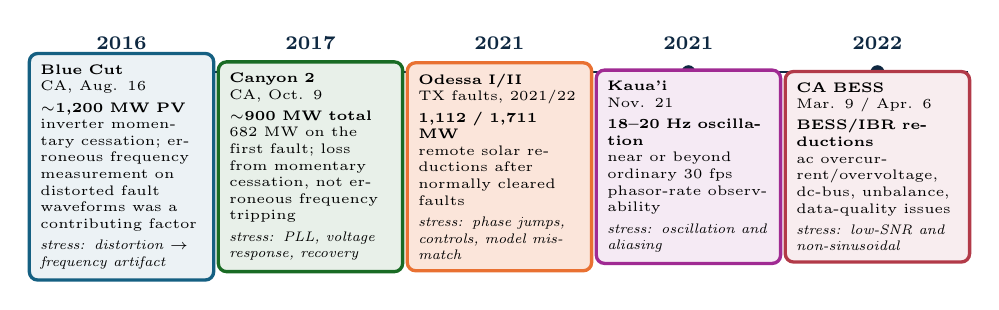
\begin{tikzpicture}[
  x=1cm,y=1cm,
  event/.style={draw, rounded corners=3pt, very thick, align=left, text width=2.06cm, minimum height=2.25cm, inner sep=4pt, font=\tiny},
  dot/.style={circle, fill=ofbInk, inner sep=1.8pt},
  link/.style={thick, color=ofbInk},
  tag/.style={font=\scriptsize\bfseries, color=ofbInk}
]
\draw[link] (-0.25,0.05) -- (11.35,0.05);

\node[dot] at (0.6,0.05) {};
\node[tag] at (0.6,0.42) {2016};
\node[event, fill=ofbBlue!8, draw=ofbBlue] at (0.6,-1.15) {
\textbf{Blue Cut}\\
CA, Aug. 16\\[0.25em]
\textbf{$\sim$1,200 MW PV}\\
inverter momentary cessation; erroneous frequency measurement on distorted fault waveforms was a contributing factor\\[0.25em]
\textit{stress: distortion $\rightarrow$ frequency artifact}
};

\node[dot] at (3.0,0.05) {};
\node[tag] at (3.0,0.42) {2017};
\node[event, fill=ofbGreen!10, draw=ofbGreen] at (3.0,-1.15) {
\textbf{Canyon 2}\\
CA, Oct. 9\\[0.25em]
\textbf{$\sim$900 MW total}\\
682 MW on the first fault; loss from momentary cessation, not erroneous frequency tripping\\[0.25em]
\textit{stress: PLL, voltage response, recovery}
};

\node[dot] at (5.4,0.05) {};
\node[tag] at (5.4,0.42) {2021};
\node[event, fill=ofbGold!18, draw=ofbGold] at (5.4,-1.15) {
\textbf{Odessa I/II}\\
TX faults, 2021/22\\[0.25em]
\textbf{1,112 / 1,711 MW}\\
remote solar reductions after normally cleared faults\\[0.25em]
\textit{stress: phase jumps, controls, model mismatch}
};

\node[dot] at (7.8,0.05) {};
\node[tag] at (7.8,0.42) {2021};
\node[event, fill=ofbViolet!10, draw=ofbViolet] at (7.8,-1.15) {
\textbf{Kaua'i}\\
Nov. 21\\[0.25em]
\textbf{18--20 Hz oscillation}\\
near or beyond ordinary 30 fps phasor-rate observability\\[0.25em]
\textit{stress: oscillation and aliasing}
};

\node[dot] at (10.2,0.05) {};
\node[tag] at (10.2,0.42) {2022};
\node[event, fill=ofbRed!9, draw=ofbRed] at (10.2,-1.15) {
\textbf{CA BESS}\\
Mar. 9 / Apr. 6\\[0.25em]
\textbf{BESS/IBR reductions}\\
ac overcurrent/overvoltage, dc-bus, unbalance, data-quality issues\\[0.25em]
\textit{stress: low-SNR and non-sinusoidal}
};
\end{tikzpicture}
\end{center}
\vspace{-0.2em}
\callout{\textbf{Benchmark implication:} the estimator must be tested against waveform distortion, phase jumps, control recovery, unbalance, noise, harmonics, interharmonics, and reporting-rate limits, not only steady-state frequency error.}
\artifact{NERC/WECC Blue Cut (2017); 900~MW Canyon 2 (2018); NERC Odessa I/II (2021, 2022); NERC/WECC CA BESS (2023); Dong et al., Kaua'i 18--20~Hz oscillations (arXiv:2301.05781)}
\end{frame}

\begin{frame}[label=researchproblem]{Research problem}
\begin{columns}[T,onlytextwidth]
\column{0.55\linewidth}
\begin{itemize}
  \item Low-inertia IBR grids require reliable local frequency estimates during ramps, phase jumps, harmonic distortion, ringdown, and mixed dynamic events.
  \item Classical estimators often trade off responsiveness, noise rejection, latency, and computational load.
  \item Modern model-based and data-driven estimators improve some regimes, but can be difficult to compare fairly.
  \item Existing comparisons often under-specify seeds, disturbance families, tuning policy, trip-risk, structural latency, or computational cost.
\end{itemize}
\column{0.40\linewidth}
\begin{block}{Research gap}
The literature needs a reproducible benchmark that connects estimator error to protection-oriented risk, settling behavior, and deployability.
\end{block}
\end{columns}
\end{frame}

\begin{frame}[label=technicalcontributions]{Technical contributions}
\vspace{-0.25em}
\centering
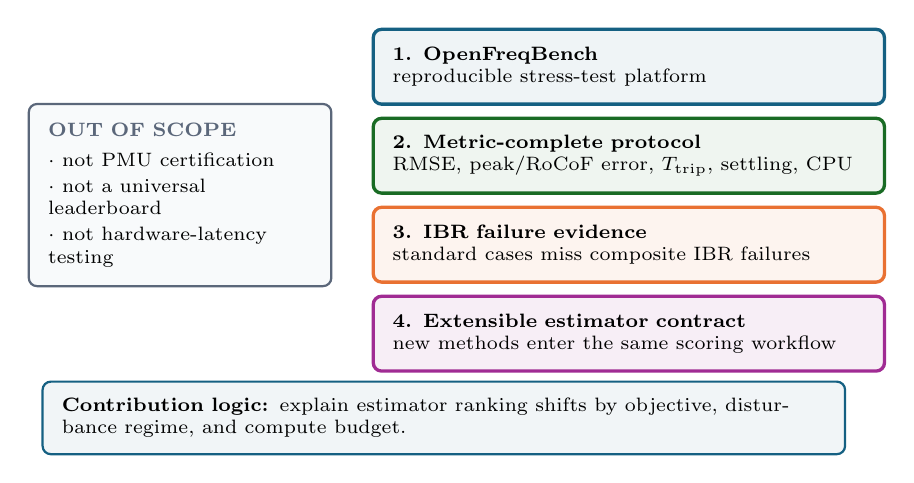
\begin{tikzpicture}[
  every node/.style={font=\scriptsize},
  contrib/.style={draw, rounded corners=3pt, very thick, align=left, text width=6.0cm, minimum height=0.95cm, inner xsep=7pt, inner ysep=5pt}
]
% Left: one neutral "out of scope" card (uniform muted -> no color clash with contributions)
\node[draw=ofbMuted, fill=cardFill, rounded corners=3pt, line width=0.8pt, align=left, text width=3.35cm, inner xsep=7pt, inner ysep=7pt] (scope) at (1.65,-0.45) {%
\hyphenpenalty=10000\exhyphenpenalty=10000\relax
{\bfseries\color{ofbMuted}OUT OF SCOPE}\\[0.35em]
$\cdot$~not PMU certification\\[0.18em]
$\cdot$~not a universal leaderboard\\[0.18em]
$\cdot$~not hardware-latency testing%
};
% Right: four contributions, distinct accents, comfortable vertical spacing
\node[contrib, fill=ofbBlue!7, draw=ofbBlue]    (c1) at (7.35,1.18)  {\textbf{1. OpenFreqBench}\\reproducible stress-test platform};
\node[contrib, fill=ofbGreen!7, draw=ofbGreen]   (c2) at (7.35,0.05)  {\textbf{2. Metric-complete protocol}\\RMSE, peak/RoCoF error, $T_{\mathrm{trip}}$, settling, CPU};
\node[contrib, fill=ofbRust!8, draw=ofbRust]     (c3) at (7.35,-1.08) {\textbf{3. IBR failure evidence}\\standard cases miss composite IBR failures};
\node[contrib, fill=ofbViolet!8, draw=ofbViolet] (c4) at (7.35,-2.21) {\textbf{4. Extensible estimator contract}\\new methods enter the same scoring workflow};
\node[draw=ofbBlue, fill=ofbBlue!6, rounded corners=3pt, line width=0.8pt, align=left, text width=9.7cm, inner xsep=7pt, inner ysep=6pt] at (5.0,-3.28) {%
\textbf{Contribution logic:} explain estimator ranking shifts by objective, disturbance regime, and compute budget.};
\end{tikzpicture}
\end{frame}

\section{Benchmark}
\sectionframe{}{Benchmark \& Platform}{An open, reproducible estimator benchmark}

\begin{frame}[label=openfreqbenchplatform]{OpenFreqBench platform}
\vspace{-0.25em}
\begin{center}
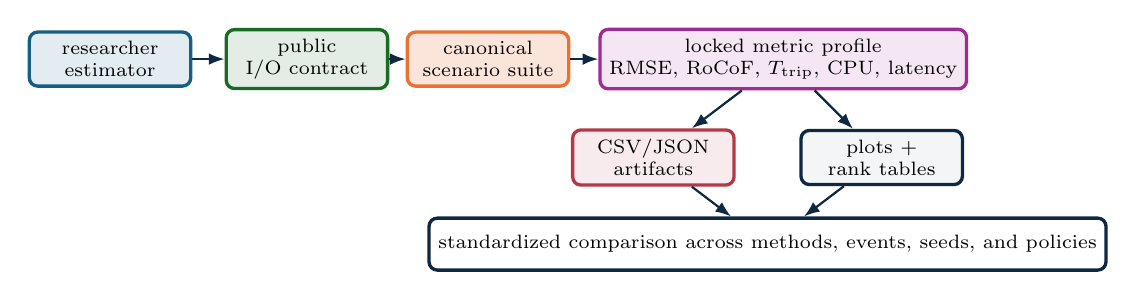
\begin{tikzpicture}[
  every node/.style={font=\scriptsize},
  box/.style={draw, rounded corners=3pt, very thick, align=center, minimum width=2.05cm, minimum height=0.66cm},
  wide/.style={draw, rounded corners=3pt, very thick, align=center, minimum width=4.55cm, minimum height=0.66cm},
  arr/.style={-{Latex[length=2mm]}, thick, color=ofbInk}
]
\node[box, fill=ofbBlue!12, draw=ofbBlue] (method) at (0,1.10) {researcher\\estimator};
\node[box, fill=ofbGreen!12, draw=ofbGreen] (api) at (2.50,1.10) {public\\I/O contract};
\node[box, fill=ofbGold!18, draw=ofbGold] (scen) at (4.80,1.10) {canonical\\scenario suite};
\node[wide, fill=ofbViolet!12, draw=ofbViolet, minimum width=4.2cm] (metrics) at (8.55,1.10) {locked metric profile\\RMSE, RoCoF, $T_{\mathrm{trip}}$, CPU, latency};
\node[box, fill=ofbRed!10, draw=ofbRed] (art) at (6.90,-0.15) {CSV/JSON\\artifacts};
\node[box, fill=ofbSoft, draw=ofbInk] (plots) at (9.80,-0.15) {plots +\\rank tables};
\node[wide, fill=white, draw=ofbInk] (compare) at (8.35,-1.25) {standardized comparison across methods, events, seeds, and policies};
\draw[arr] (method) -- (api);
\draw[arr] (api) -- (scen);
\draw[arr] (scen) -- (metrics);
\draw[arr] (metrics) -- (art);
\draw[arr] (metrics) -- (plots);
\draw[arr] (art) -- (compare);
\draw[arr] (plots) -- (compare);
\end{tikzpicture}
\end{center}
\vspace{-0.25em}
\begin{columns}[T,onlytextwidth]
\column{0.31\linewidth}
\begin{block}{Researchers add}
\scriptsize
Estimator code, parameters, and hypotheses through the public contract.
\end{block}
\column{0.33\linewidth}
\begin{block}{Platform fixes}
\scriptsize
Truth signals, sampling, seeds, tuning policy, metric formulas, and schema.
\end{block}
\column{0.31\linewidth}
\begin{block}{Outputs}
\scriptsize
Benchmark reports, metric tables, plots, manifests, and readiness gates.
\end{block}
\end{columns}
\vspace{0.05em}
{\scriptsize\color{ofbInk}\textbf{Principle:} a submitted estimator becomes a repeatable benchmark entry under the same scenarios, seeds, metrics, and artifacts.}
\end{frame}

\begin{frame}[label=experimentscale]{Experiment scale}
\centering
\vspace{0.45em}
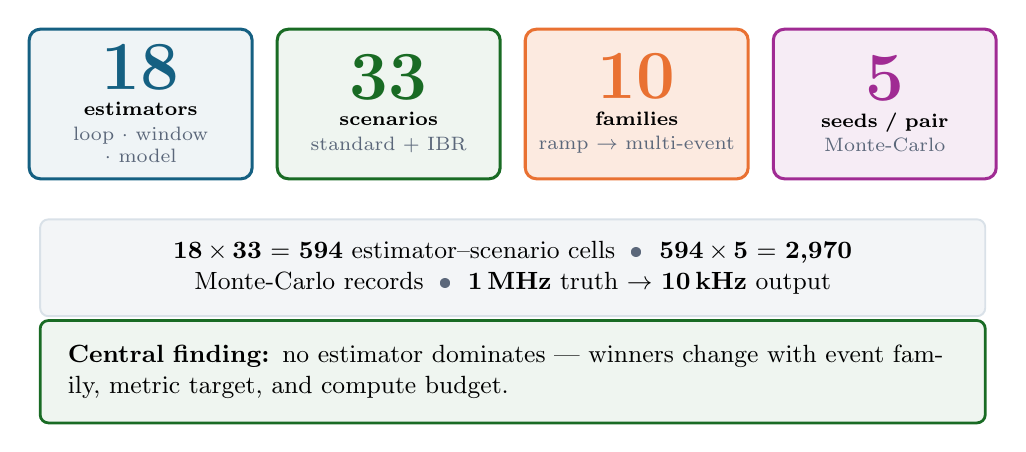
\begin{tikzpicture}[
  every node/.style={font=\scriptsize},
  hero/.style={draw, rounded corners=4pt, line width=1.1pt, align=center, text width=2.55cm, minimum height=1.9cm, inner sep=4pt, execute at begin node={\hyphenpenalty=10000\exhyphenpenalty=10000}},
  strip/.style={draw, rounded corners=3pt, line width=0.7pt, align=center, inner xsep=10pt, inner ysep=8pt, font=\small},
  take/.style={draw, rounded corners=3pt, line width=1.0pt, align=left, inner xsep=10pt, inner ysep=9pt, font=\small}
]
\node[hero, fill=ofbBlue!7, draw=ofbBlue]     (e) at (0,1.30)    {{\fontsize{25}{27}\selectfont\bfseries\color{ofbBlue}18}\\[0.20em]\textbf{estimators}\\[0.12em]{\color{ofbMuted}loop $\cdot$ window $\cdot$ model}};
\node[hero, fill=ofbGreen!7, draw=ofbGreen]   (s) at (3.15,1.30) {{\fontsize{25}{27}\selectfont\bfseries\color{ofbGreen}33}\\[0.20em]\textbf{scenarios}\\[0.12em]{\color{ofbMuted}standard $+$ IBR}};
\node[hero, fill=ofbGold!15, draw=ofbGold]    (f) at (6.30,1.30) {{\fontsize{25}{27}\selectfont\bfseries\color{ofbGold}10}\\[0.20em]\textbf{families}\\[0.12em]{\color{ofbMuted}ramp $\to$ multi-event}};
\node[hero, fill=ofbViolet!9, draw=ofbViolet] (m) at (9.45,1.30) {{\fontsize{25}{27}\selectfont\bfseries\color{ofbViolet}5}\\[0.20em]\textbf{seeds / pair}\\[0.12em]{\color{ofbMuted}Monte-Carlo}};

\node[strip, fill=ofbSoft, draw=ofbLine, text width=11.3cm] (d) at (4.725,-0.78) {%
\textbf{18\,\(\times\)\,33 \(=\) 594} estimator--scenario cells \;\textcolor{ofbMuted}{\textbullet}\; \textbf{594\,\(\times\)\,5 \(=\) 2{,}970} Monte-Carlo records \;\textcolor{ofbMuted}{\textbullet}\; \textbf{1\,MHz} truth \(\to\) \textbf{10\,kHz} output%
};

\node[take, fill=ofbGreen!7, draw=ofbGreen, text width=11.3cm] (t) at (4.725,-2.10) {%
\textbf{Central finding:} no estimator dominates --- winners change with event family, metric target, and compute budget.%
};
\end{tikzpicture}
\vspace{0.25em}
\artifact{OpenFreqBench expanded scenario matrix}
\end{frame}

\begin{frame}[label=estimatorfamilies]{Estimator families}
\begin{columns}[T,onlytextwidth]
\column{0.30\linewidth}
\begin{block}{Loop-based}
\small
PLL, SOGI-PLL, SOGI-FLL, Type-3 SOGI-PLL.
\end{block}
\begin{block}{Window / spectral}
\small
IpDFT, TFT, ESPRIT, Prony, MUSIC.
\end{block}
\column{0.31\linewidth}
\begin{block}{Model-based / stochastic}
\small
EKF, UKF, RA-EKF, LKF, LKF2.
\end{block}
\begin{block}{Adaptive and data-driven}
\small
RLS, Koopman (RK-DPMU).
\end{block}
\column{0.33\linewidth}
\begin{block}{Legacy baselines}
\small
TKEO and ZCD are retained as comparison references outside the recommended deployment set.
\end{block}
\begin{block}{Interpretation rule}
\small
These families occupy different latency and stress-sensitivity positions. The comparison tracks where each family wins, degrades, and fails.
\end{block}
\end{columns}
\vspace{0.3em}
{\scriptsize\color{ofbMuted}LKF and LKF2 follow H.~Ahmed, S.~Biricik, M.~Benbouzid, ``Linear Kalman Filter-Based Grid Synchronization Technique: An Alternative Implementation,'' IEEE, 2021.}
\end{frame}

\section{Scenarios}
\sectionframe{}{Scenarios}{Standard and composite IBR stress cases}

{\setbeamerfont{frametitle}{family=\rmfamily,series=\mdseries,size=\fontsize{14}{16.5}\selectfont}
\begin{frame}[label=standardstresses]{Standard stress scenarios}
\vspace{-0.05em}
\evidencetag{ofbBlue}{CORE SCENARIO SUITE}
\begin{center}
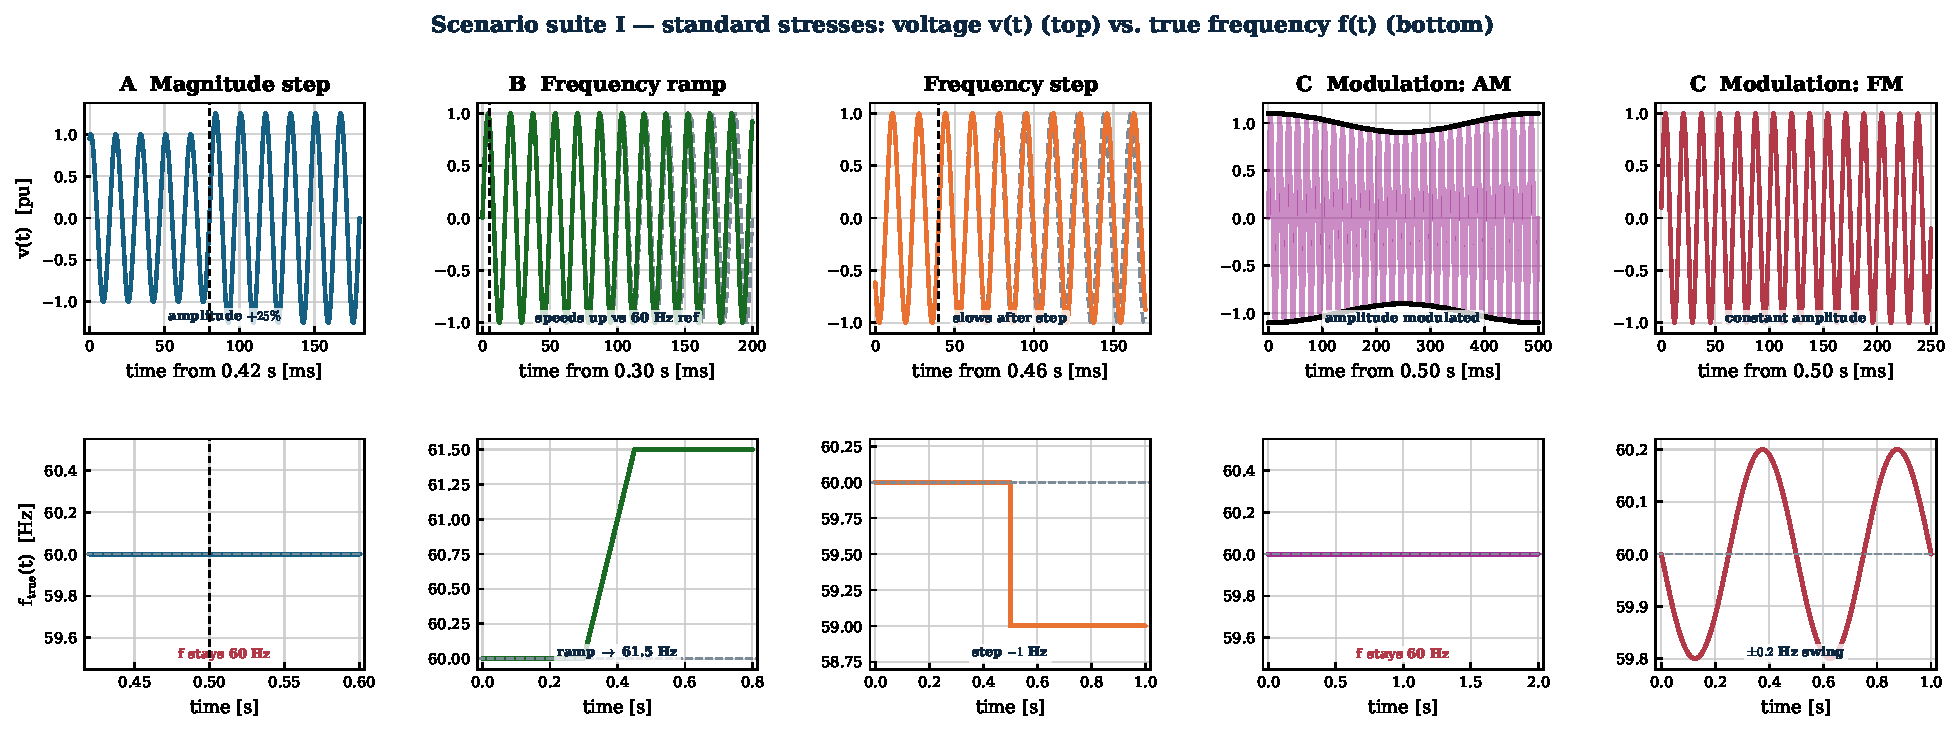
\includegraphics[width=0.99\linewidth,height=0.70\textheight,keepaspectratio]{figures/scenario_suite_1.pdf}
\end{center}
\end{frame}
}

{\setbeamerfont{frametitle}{family=\rmfamily,series=\mdseries,size=\fontsize{14}{16.5}\selectfont}
\begin{frame}[label=ibrstresses]{Composite IBR stress scenarios}
\vspace{-0.05em}
\evidencetag{ofbRust}{IBR STRESS SUITE}
\begin{center}
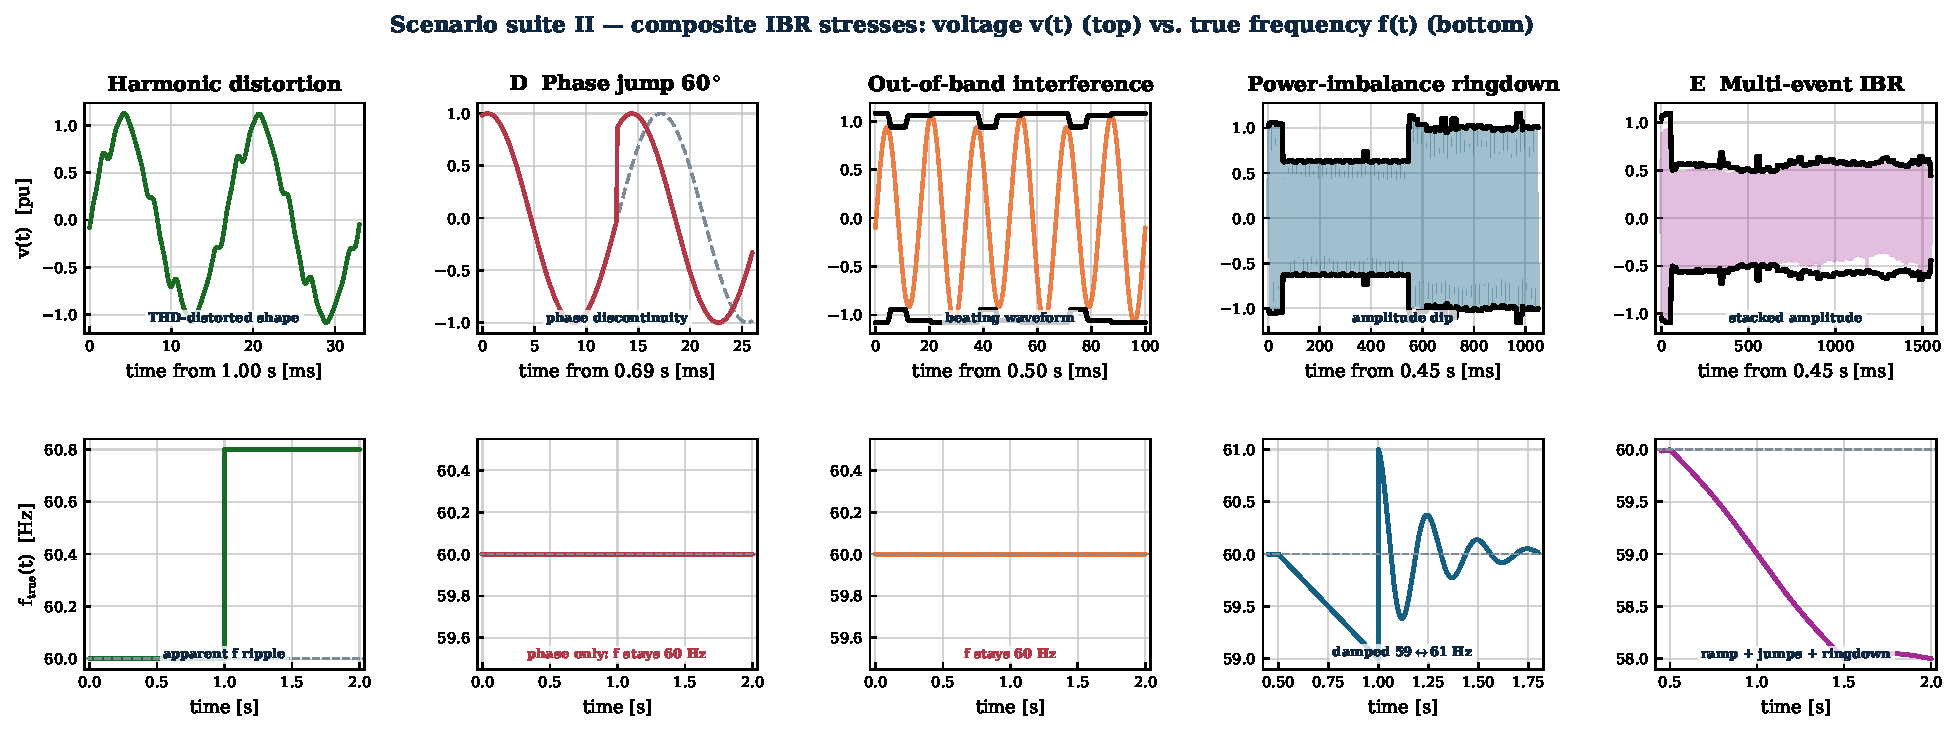
\includegraphics[width=0.99\linewidth,height=0.70\textheight,keepaspectratio]{figures/scenario_suite_2.pdf}
\end{center}
\end{frame}
}

\section{Method}
\sectionframe{}{Metrics \& Methodology}{How every estimator is measured}

\begin{frame}[label=experimentalmethod]{Experimental method}
\vspace{-0.35em}
\centering
\resizebox{0.98\linewidth}{!}{%
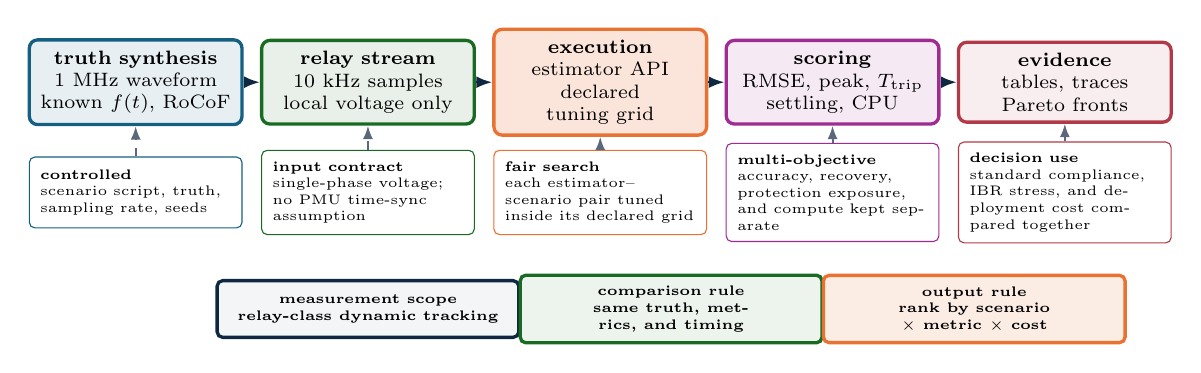
\begin{tikzpicture}[
  every node/.style={font=\scriptsize},
  lane/.style={draw, rounded corners=3pt, very thick, align=center, text width=2.42cm, minimum height=0.92cm, inner sep=4pt},
  note/.style={draw, rounded corners=2pt, align=left, text width=2.42cm, minimum height=0.90cm, inner sep=4pt, font=\tiny},
  gate/.style={draw, rounded corners=2pt, very thick, align=center, text width=3.55cm, minimum height=0.72cm, inner sep=4pt, font=\tiny\bfseries},
  arr/.style={-{Latex[length=2mm]}, line width=0.9pt, color=ofbInk},
  weak/.style={-{Latex[length=1.7mm]}, line width=0.7pt, dashed, color=ofbMuted}
]
\node[lane, fill=ofbBlue!10, draw=ofbBlue] (truth) at (0,1.30) {\textbf{truth synthesis}\\1 MHz waveform\\known $f(t)$, RoCoF};
\node[lane, fill=ofbGreen!10, draw=ofbGreen] (stream) at (2.95,1.30) {\textbf{relay stream}\\10 kHz samples\\local voltage only};
\node[lane, fill=ofbGold!18, draw=ofbGold] (exec) at (5.90,1.30) {\textbf{execution}\\estimator API\\declared tuning grid};
\node[lane, fill=ofbViolet!10, draw=ofbViolet] (score) at (8.85,1.30) {\textbf{scoring}\\RMSE, peak, $T_{\mathrm{trip}}$\\settling, CPU};
\node[lane, fill=ofbRed!9, draw=ofbRed] (rank) at (11.80,1.30) {\textbf{evidence}\\tables, traces\\Pareto fronts};
\draw[arr] (truth) -- (stream);
\draw[arr] (stream) -- (exec);
\draw[arr] (exec) -- (score);
\draw[arr] (score) -- (rank);

\node[note, fill=white, draw=ofbBlue] (c1) at (0,-0.10) {\textbf{controlled}\\scenario script, truth, sampling rate, seeds};
\node[note, fill=white, draw=ofbGreen] (c2) at (2.95,-0.10) {\textbf{input contract}\\single-phase voltage; no PMU time-sync assumption};
\node[note, fill=white, draw=ofbGold] (c3) at (5.90,-0.10) {\textbf{fair search}\\each estimator--scenario pair tuned inside its declared grid};
\node[note, fill=white, draw=ofbViolet] (c4) at (8.85,-0.10) {\textbf{multi-objective}\\accuracy, recovery, protection exposure, and compute kept separate};
\node[note, fill=white, draw=ofbRed] (c5) at (11.80,-0.10) {\textbf{decision use}\\standard compliance, IBR stress, and deployment cost compared together};
\draw[weak] (c1) -- (truth);
\draw[weak] (c2) -- (stream);
\draw[weak] (c3) -- (exec);
\draw[weak] (c4) -- (score);
\draw[weak] (c5) -- (rank);

\node[gate, fill=ofbSoft, draw=ofbInk] at (2.95,-1.58) {measurement scope\\relay-class dynamic tracking};
\node[gate, fill=ofbGreen!8, draw=ofbGreen] at (6.80,-1.58) {comparison rule\\same truth, metrics, and timing};
\node[gate, fill=ofbGold!13, draw=ofbGold] at (10.65,-1.58) {output rule\\rank by scenario $\times$ metric $\times$ cost};
\end{tikzpicture}%
}
\vspace{-0.05em}
\end{frame}

\begin{frame}[label=fullworkflow]{Full benchmark workflow}
\centering
\vspace{-0.35em}
\resizebox{0.985\textwidth}{!}{%
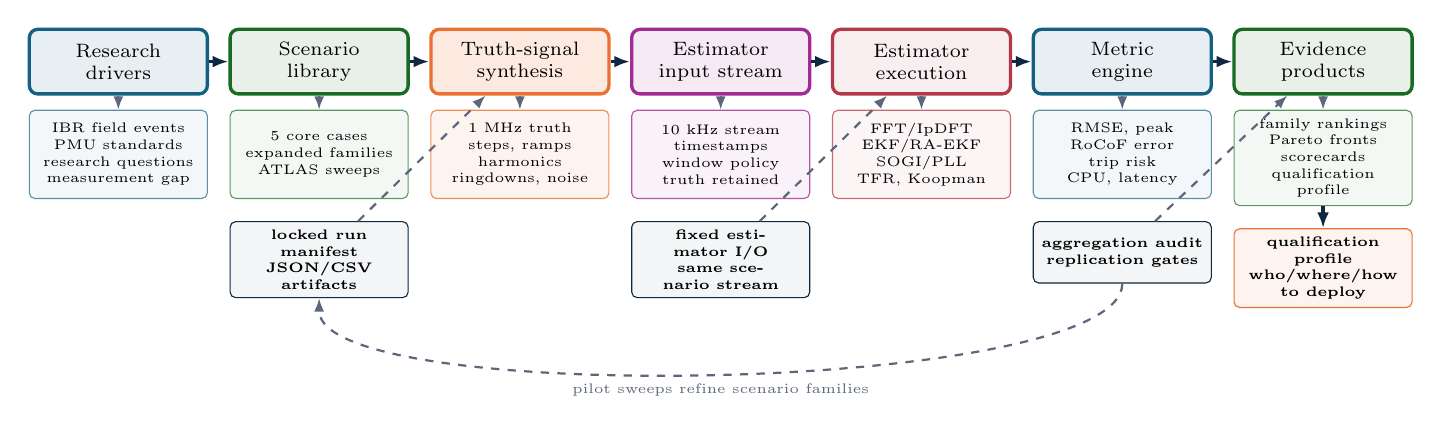
\begin{tikzpicture}[
  every node/.style={font=\scriptsize},
  stage/.style={draw, rounded corners=3pt, very thick, align=center, text width=2.05cm, minimum height=0.82cm, inner sep=3pt},
  detail/.style={draw, rounded corners=2pt, align=center, text width=2.05cm, minimum height=1.12cm, inner sep=3pt, font=\tiny},
  gate/.style={draw, rounded corners=2pt, align=center, text width=2.05cm, minimum height=0.78cm, inner sep=3pt, font=\tiny\bfseries},
  main/.style={-{Latex[length=2.0mm]}, very thick, color=ofbInk},
  aux/.style={-{Latex[length=1.7mm]}, thick, dashed, color=ofbMuted}
]
\node[stage, draw=ofbBlue, fill=ofbBlue!10] (drivers) at (0,2.8) {Research\\drivers};
\node[stage, draw=ofbGreen, fill=ofbGreen!10] (scenario) at (2.55,2.8) {Scenario\\library};
\node[stage, draw=ofbGold, fill=ofbGold!15] (truth) at (5.10,2.8) {Truth-signal\\synthesis};
\node[stage, draw=ofbViolet, fill=ofbViolet!10] (stream) at (7.65,2.8) {Estimator\\input stream};
\node[stage, draw=ofbRed, fill=ofbRed!9] (estimators) at (10.20,2.8) {Estimator\\execution};
\node[stage, draw=ofbBlue, fill=ofbBlue!10] (metrics) at (12.75,2.8) {Metric\\engine};
\node[stage, draw=ofbGreen, fill=ofbGreen!10] (evidence) at (15.30,2.8) {Evidence\\products};

\node[detail, draw=ofbBlue!70, fill=ofbBlue!5, below=0.18cm of drivers] (dDrivers)
{IBR field events\\PMU standards\\research questions\\measurement gap};
\node[detail, draw=ofbGreen!70, fill=ofbGreen!5, below=0.18cm of scenario] (dScenario)
{5 core cases\\expanded families\\ATLAS sweeps};
\node[detail, draw=ofbGold!80, fill=ofbGold!8, below=0.18cm of truth] (dTruth)
{1 MHz truth\\steps, ramps\\harmonics\\ringdowns, noise};
\node[detail, draw=ofbViolet!80, fill=ofbViolet!6, below=0.18cm of stream] (dStream)
{10 kHz stream\\timestamps\\window policy\\truth retained};
\node[detail, draw=ofbRed!75, fill=ofbRed!5, below=0.18cm of estimators] (dEstimators)
{FFT/IpDFT\\EKF/RA-EKF\\SOGI/PLL\\TFR, Koopman};
\node[detail, draw=ofbBlue!70, fill=ofbBlue!5, below=0.18cm of metrics] (dMetrics)
{RMSE, peak\\RoCoF error\\trip risk\\CPU, latency};
\node[detail, draw=ofbGreen!70, fill=ofbGreen!5, below=0.18cm of evidence] (dEvidence)
{family rankings\\Pareto fronts\\scorecards\\qualification profile};

\node[gate, draw=ofbInk, fill=ofbSoft, below=0.28cm of dScenario] (manifest)
{locked run manifest\\JSON/CSV artifacts};
\node[gate, draw=ofbInk, fill=ofbSoft, below=0.28cm of dStream] (contract)
{fixed estimator I/O\\same scenario stream};
\node[gate, draw=ofbInk, fill=ofbSoft, below=0.28cm of dMetrics] (audit)
{aggregation audit\\replication gates};
\node[gate, draw=ofbRust, fill=ofbRust!8, below=0.28cm of dEvidence] (profile)
{qualification profile\\who/where/how to deploy};

\draw[main] (drivers) -- (scenario);
\draw[main] (scenario) -- (truth);
\draw[main] (truth) -- (stream);
\draw[main] (stream) -- (estimators);
\draw[main] (estimators) -- (metrics);
\draw[main] (metrics) -- (evidence);

\foreach \a/\b in {drivers/dDrivers,scenario/dScenario,truth/dTruth,stream/dStream,estimators/dEstimators,metrics/dMetrics,evidence/dEvidence}
  \draw[aux] (\a) -- (\b);
\draw[aux] (manifest) -- (truth);
\draw[aux] (contract) -- (estimators);
\draw[aux] (audit) -- (evidence);
\draw[main] (dEvidence) -- (profile);
\draw[aux] (audit.south) to[out=-90,in=-90,looseness=0.35] node[below, font=\tiny, align=center, text=ofbMuted] {pilot sweeps refine scenario families} (manifest.south);
\end{tikzpicture}%
}
\vspace{0.2em}
\callout{The benchmark is an evidence pipeline, not just a test script: every figure traces back to a locked manifest, a fixed I/O contract, and the readiness gate.}
\end{frame}

\begin{frame}[label=metrics]{Metrics and decision variables}
\small
\begin{columns}[T,onlytextwidth]
\column{0.48\linewidth}
\begin{block}{Error and recovery}
\[
e[k]=\widehat f[k]-f_{\mathrm{true}}[k]
\]
\[
\mathrm{RMSE}=\sqrt{\frac{1}{N}\sum_k e[k]^2}
\]
\[
E_{\max}=\max_k |e[k]|
\]
\end{block}
\column{0.47\linewidth}
\begin{block}{Protection-oriented risk}
\[
T_{\mathrm{trip}}=\Delta t\sum_k \mathbf{1}\{|e[k]|>0.5\ \mathrm{Hz}\}
\]
\[
t_s=\min\{t:\ |e[\tau]|\leq \epsilon,\ \forall \tau\geq t\}
\]
\[
C_{\mathrm{CPU}}=\mathrm{mean\ time/sample}
\]
\end{block}
\end{columns}
\vspace{0.2em}
\callout{The 0.5 Hz threshold is a protection-oriented risk proxy. The metric set separates average error, transient severity, trip exposure, settling, and compute cost.}
\end{frame}

\section{Results}
\sectionframe{}{Results}{Winners depend on the question}

\begin{frame}[label=standardresults]{Standard scenario results}
\begin{columns}[T,onlytextwidth]
\column{0.58\linewidth}
\scriptsize
\renewcommand{\arraystretch}{1.18}
\setlength{\tabcolsep}{4pt}
\begin{tabular}{>{\bfseries\raggedright\arraybackslash}p{0.23\linewidth}ccc}
\toprule
Method & Step & Ramp & Mod. \\
\midrule
RA-EKF & \cellcolor{ofbGreen!25}0.000 & \cellcolor{ofbGreen!35}\textbf{0.006} & \cellcolor{ofbGreen!25}0.037 \\
SOGI-FLL & \cellcolor{ofbGreen!25}0.005 & \cellcolor{ofbGreen!25}0.013 & \cellcolor{ofbGreen!25}0.040 \\
Koopman & \cellcolor{ofbGreen!25}0.003 & \cellcolor{ofbGreen!25}0.017 & \cellcolor{ofbGreen!25}0.044 \\
TFT & \cellcolor{ofbGreen!25}0.001 & \cellcolor{ofbGreen!25}0.019 & \cellcolor{ofbGreen!25}0.046 \\
UKF & \cellcolor{ofbGreen!25}0.000 & \cellcolor{ofbGreen!25}0.017 & \cellcolor{ofbGold!22}0.055 \\
LKF2 & \cellcolor{ofbRed!18}0.138 & \cellcolor{ofbGreen!25}0.015 & \cellcolor{ofbGreen!35}\textbf{0.028} \\
\only<2->{PLL} & \only<2->{\cellcolor{ofbGreen!25}0.033} & \only<2->{\cellcolor{ofbRed!25}\textbf{1.47}} & \only<2->{\cellcolor{ofbRed!25}\textbf{0.227}} \\
\only<2->{IpDFT} & \only<2->{\cellcolor{ofbGreen!25}0.000} & \only<2->{\cellcolor{ofbRed!35}\textbf{14.4}} & \only<2->{\cellcolor{ofbRed!18}0.114} \\
\only<2->{EKF} & \only<2->{\cellcolor{ofbGreen!25}0.000} & \only<2->{\cellcolor{ofbRed!35}\textbf{37.1}} & \only<2->{\cellcolor{ofbGold!22}0.064} \\
\bottomrule
\end{tabular}
\vspace{0.15em}
{\tiny\color{ofbMuted}RMSE [Hz], mean over 5 seeds. Green: below 0.05 Hz guide; red: failure/divergence regime.\\[0.25em]LKF2 implementation after H.~Ahmed, S.~Biricik, M.~Benbouzid, ``Linear Kalman Filter-Based Grid Synchronization Technique: An Alternative Implementation,'' IEEE, 2021.}
\column{0.38\linewidth}
\begin{block}{What the heatmap shows}
\small
The magnitude step is easy for most methods. The ramp is the separator: windowed (IpDFT) and some filters can look excellent at a point and still diverge in another seed.
\end{block}
\begin{block}{Operational consequence}
\small
Robustness is not the same as point accuracy. A standard scenario can pass while the same estimator remains unsafe for ramp-like IBR dynamics.
\end{block}
\end{columns}
\end{frame}

\begin{frame}[label=compositeibr]{Composite IBR sequence: why it is hardest}
\vspace{0.1em}
\begin{center}
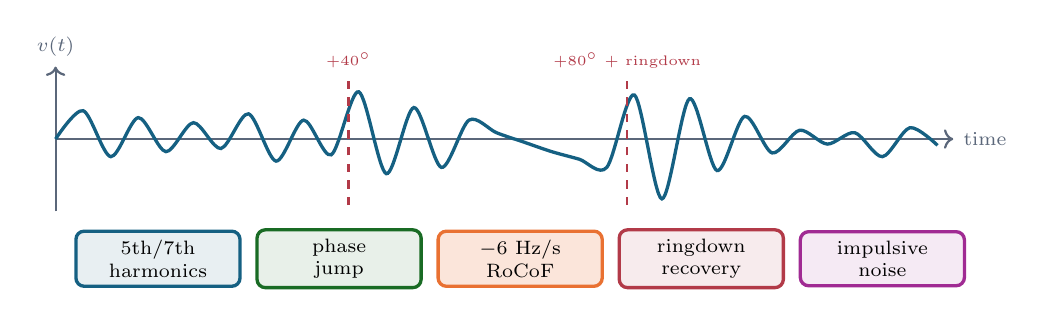
\begin{tikzpicture}[
  x=1cm,y=0.8cm,
  stress/.style={draw, rounded corners=3pt, very thick, align=center, text width=1.85cm, minimum height=0.66cm, font=\scriptsize},
  arr/.style={-{Latex[length=2mm]}, thick, color=ofbInk},
  axis/.style={thick, color=ofbMuted}
]
\draw[axis, ->] (0,0) -- (11.4,0) node[right,font=\scriptsize] {time};
\draw[axis, ->] (0,-1.15) -- (0,1.15) node[above,font=\scriptsize] {$v(t)$};
\draw[ofbBlue, very thick, smooth] plot coordinates {
  (0,0) (0.35,0.45) (0.70,-0.28) (1.05,0.34) (1.40,-0.20) (1.75,0.26)
  (2.10,-0.15) (2.45,0.40) (2.80,-0.35) (3.15,0.30) (3.50,-0.25)
  (3.85,0.75) (4.20,-0.55) (4.55,0.50) (4.90,-0.45) (5.25,0.30)
  (5.60,0.10) (5.95,-0.05) (6.30,-0.20) (6.65,-0.32) (7.00,-0.45)
  (7.35,0.70) (7.70,-0.95) (8.05,0.64) (8.40,-0.50) (8.75,0.36)
  (9.10,-0.22) (9.45,0.14) (9.80,-0.08) (10.15,0.10) (10.50,-0.28)
  (10.85,0.18) (11.20,-0.10)
};
\draw[dashed, ofbRed, thick] (3.72,-1.05) -- (3.72,1.05);
\draw[dashed, ofbRed, thick] (7.26,-1.05) -- (7.26,1.05);
\node[font=\tiny, ofbRed] at (3.72,1.25) {$+40^\circ$};
\node[font=\tiny, ofbRed] at (7.26,1.25) {$+80^\circ$ + ringdown};

\node[stress, fill=ofbBlue!10, draw=ofbBlue] at (1.3,-1.9) {5th/7th\\harmonics};
\node[stress, fill=ofbGreen!10, draw=ofbGreen] at (3.6,-1.9) {phase\\jump};
\node[stress, fill=ofbGold!18, draw=ofbGold] at (5.9,-1.9) {$-6$ Hz/s\\RoCoF};
\node[stress, fill=ofbRed!10, draw=ofbRed] at (8.2,-1.9) {ringdown\\recovery};
\node[stress, fill=ofbViolet!10, draw=ofbViolet] at (10.5,-1.9) {impulsive\\noise};
\end{tikzpicture}
\end{center}
\vspace{0.6em}
\begin{columns}[T,onlytextwidth]
\column{0.48\linewidth}
\begin{block}{Why standard tests miss it}
\scriptsize
The estimator sees spectral leakage, loop re-lock, state-model mismatch, transient recovery, and noise in one nonstationary waveform.
\end{block}
\column{0.47\linewidth}
\begin{block}{Why ATLAS decomposes it}
\scriptsize
The multi-event case proves the failure exists; severity sweeps identify which stressor actually breaks each estimator family.
\end{block}
\end{columns}
\end{frame}

\begin{frame}{Scenario E: the leaderboard breaks}
\scriptsize
\setlength{\tabcolsep}{7pt}
\renewcommand{\arraystretch}{1.14}
\begin{center}
\begin{tabular}{>{\bfseries\raggedright\arraybackslash}p{0.20\linewidth}rrr}
\toprule
Method & RMSE [Hz] & $T_{\mathrm{trip}}$ [s] & CPU [$\mu$s] \\
\midrule
UKF & \textbf{1.09} & \textbf{0.78} & 14 \\
EKF & 1.13 & 0.87 & 11 \\
SOGI-PLL & 1.14 & \textbf{0.78} & 11 \\
SOGI-FLL & 1.14 & 0.84 & \textbf{9} \\
IpDFT & 1.14 & 1.35 & 17 \\
RA-EKF & 1.16 & 0.92 & 15 \\
Koopman & 1.90 & 0.84 & \textbf{15\,241} \\
ZCD & \textbf{$>$400} & 1.55 & 7 \\
\bottomrule
\end{tabular}
\end{center}
\vspace{0.25em}
\begin{columns}[T,onlytextwidth]
\column{0.48\linewidth}
\begin{block}{No accurate winner}
\small
Under the stacked sequence every usable method collapses to $\approx1.1$ Hz RMSE; ZCD diverges catastrophically (hundreds of Hz, strongly seed-dependent). High accuracy is simply not available here.
\end{block}
\column{0.47\linewidth}
\begin{block}{Scalar ranking failure}
\small
UKF has the lowest RMSE and trip exposure, SOGI-FLL the lowest usable CPU, Koopman is $1000\times$ costlier; RA-EKF sits mid-pack but never diverges.
\end{block}
\end{columns}
\artifact{Monte-Carlo benchmark, $n=5$ seeds --- composite multi-event scenario}
\end{frame}

\begin{frame}[label=resultcomparison]{Result comparison: winners depend on the question}
\scriptsize
\setlength{\tabcolsep}{5pt}
\renewcommand{\arraystretch}{1.16}
\begin{center}
\resizebox{0.98\linewidth}{!}{%
\begin{tabular}{>{\bfseries\raggedright\arraybackslash}p{0.22\linewidth}>{\raggedright\arraybackslash}p{0.23\linewidth}>{\raggedright\arraybackslash}p{0.20\linewidth}>{\raggedright\arraybackslash}p{0.27\linewidth}}
\toprule
Question & Best-supported answer & Evidence & Boundary \\
\midrule
Clean step/modulation accuracy & State-space + SOGI-FLL near-zero; LKF2 best on mod & Step $\approx0$; mod 0.028--0.044 Hz & Clean cases do not predict ramp/event survival \\
Ramp and RoCoF tracking & RA-EKF is the most robust ramp tracker & 0.006 Hz; windowed IpDFT 14 Hz diverges & Some filters show intermittent seed-dependent blow-ups \\
Phase jump (Scenario D) & State-space filters recover with zero trip & EKF/UKF/RA-EKF $T_{\mathrm{trip}}=0$; IpDFT 1.21 s & Windowed/spectral carry the exposure \\
Multi-event RMSE & No accurate method --- all $\approx1.1$ Hz & UKF 1.09 Hz best; ZCD 426 Hz diverges & RMSE hides trip-risk and $1000\times$ CPU spread \\
Embedded feasibility & PLL, SOGI-FLL, EKF, RA-EKF remain plausible & 9--17 $\mu$s/sample; Koopman $\sim$15{,}000 & Python timing is a software-cost proxy \\
\bottomrule
\end{tabular}%
}
\end{center}
\vspace{0.28em}
\callout{Selection changes with event family, objective metric, and compute envelope. A single leaderboard hides the deployment trade-off.}
\end{frame}

\begin{frame}[label=computationalfeasibility]{Computational feasibility}
\scriptsize
\setlength{\tabcolsep}{5pt}
\renewcommand{\arraystretch}{1.12}
\begin{columns}[T,onlytextwidth]
\column{0.50\linewidth}
\begin{tabular}{>{\bfseries\raggedright\arraybackslash}p{0.32\linewidth}rc}
\toprule
Method & Time/sample$^\dagger$ & Cost tier \\
\midrule
SOGI-FLL & 10 $\mu$s & low \\
SOGI-PLL & 11 $\mu$s & low \\
EKF & 12 $\mu$s & low \\
RA-EKF & \textbf{15 $\mu$s} & \textbf{low} \\
TFT / IpDFT & 12 $\mu$s & low \\
ESPRIT & 95 $\mu$s & medium \\
Koopman & 0.1--15 ms & high \\
\bottomrule
\end{tabular}\\[0.35em]
{\tiny\color{ofbMuted}$\dagger$ mean per-sample wall-clock in the Python harness (software proxy), $n=5$; Koopman/ESPRIT scale with event length.}
\column{0.46\linewidth}
\begin{block}{Deployment interpretation}
\small
CPU is a software-cost indicator from the benchmark harness, not a hardware-latency claim.
\end{block}
\begin{block}{Key comparison}
\small
The practical low-cost cluster is SOGI-FLL, SOGI-PLL, EKF, and RA-EKF. Koopman and ESPRIT sit far to the right on cost without a global RMSE gain.
\end{block}
\end{columns}
\end{frame}

\begin{frame}[label=computecost]{Accuracy costs 100--1000$\times$ more compute}
\extendedresultsbanner
\centering
{\scriptsize\color{ofbMuted}Deployable methods sit lower-left; spectral/data-driven accuracy moves right by $100$--$1000\times$ CPU.}
\vspace{0.05em}
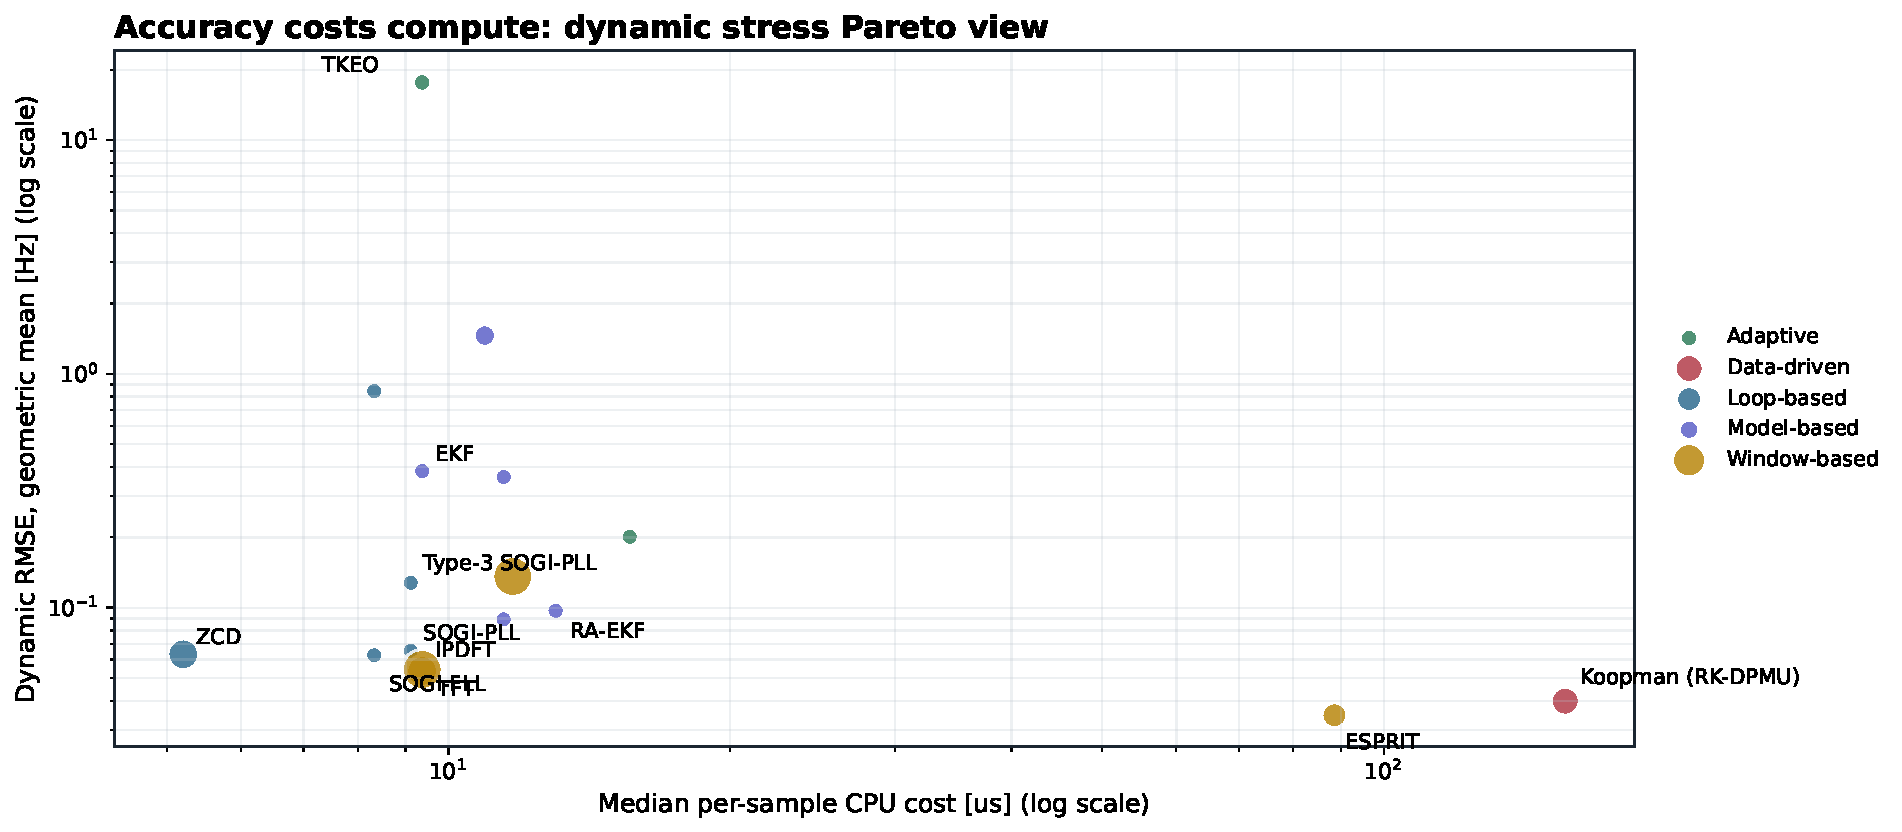
\includegraphics[width=0.99\linewidth,height=0.69\textheight,keepaspectratio]{figures/cpu_accuracy_pareto_wide.pdf}
\end{frame}

\begin{frame}[label=atlasseverity]{ATLAS severity analysis}
\papergradebanner
\begin{center}
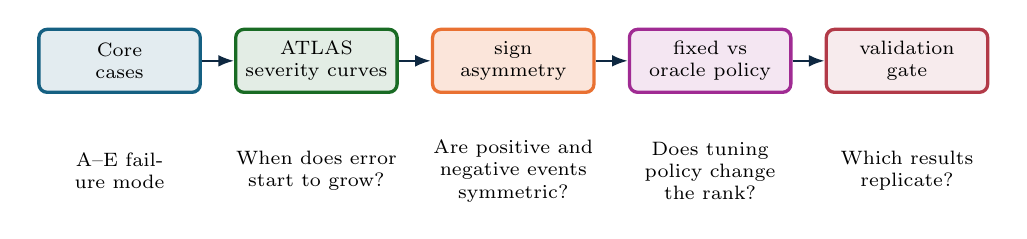
\begin{tikzpicture}[
  every node/.style={font=\scriptsize},
  box/.style={draw, rounded corners=3pt, very thick, align=center, minimum width=2.05cm, minimum height=0.80cm},
  arr/.style={-{Latex[length=2mm]}, thick, color=ofbInk}
]
\node[box, fill=ofbBlue!12, draw=ofbBlue] (paper) at (0,1.15) {Core\\cases};
\node[box, fill=ofbGreen!12, draw=ofbGreen] (sev) at (2.5,1.15) {ATLAS\\severity curves};
\node[box, fill=ofbGold!18, draw=ofbGold] (sign) at (5.0,1.15) {sign\\asymmetry};
\node[box, fill=ofbViolet!12, draw=ofbViolet] (policy) at (7.5,1.15) {fixed vs\\oracle policy};
\node[box, fill=ofbRed!10, draw=ofbRed] (gate) at (10.0,1.15) {validation\\gate};
\draw[arr] (paper) -- (sev);
\draw[arr] (sev) -- (sign);
\draw[arr] (sign) -- (policy);
\draw[arr] (policy) -- (gate);
\node[align=center, text width=2.1cm] at (0,-0.25) {A--E failure mode};
\node[align=center, text width=2.1cm] at (2.5,-0.25) {When does error start to grow?};
\node[align=center, text width=2.1cm] at (5.0,-0.25) {Are positive and negative events symmetric?};
\node[align=center, text width=2.1cm] at (7.5,-0.25) {Does tuning policy change the rank?};
\node[align=center, text width=2.1cm] at (10.0,-0.25) {Which results replicate?};
\end{tikzpicture}
\end{center}
\vspace{0.35em}
\callout{ATLAS maps where estimator behavior changes with severity, sign, tuning policy, and replication depth.}
\end{frame}

\begin{frame}[label=wholestressspace]{Severity response: amplitude and frequency steps}
\papergradebanner
\centering
{\scriptsize\color{ofbMuted}Log--log RMSE vs.\ severity ($n=30$). Most methods rise smoothly toward the Cram\'er--Rao floor; saturated curves stay high regardless of severity.}
\vspace{0.25em}
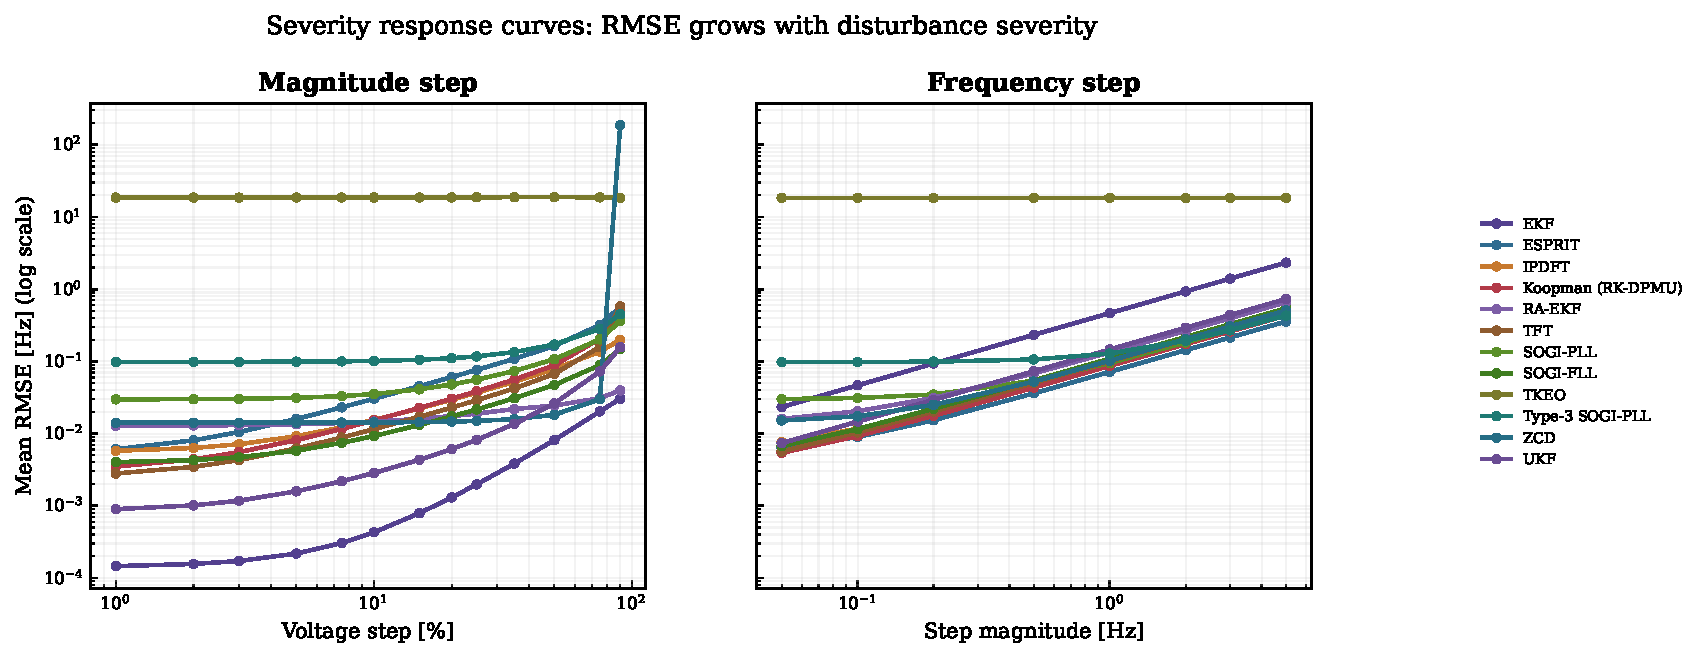
\includegraphics[width=0.97\linewidth,height=0.64\textheight,keepaspectratio]{figures/severity_curves_step.pdf}
\end{frame}

\begin{frame}{Severity response: RoCoF ramp and phase jump}
\papergradebanner
\centering
{\scriptsize\color{ofbMuted}Error grows with RoCoF magnitude and phase-jump angle; the curve slope and onset are the family-specific failure signatures.}
\vspace{0.25em}
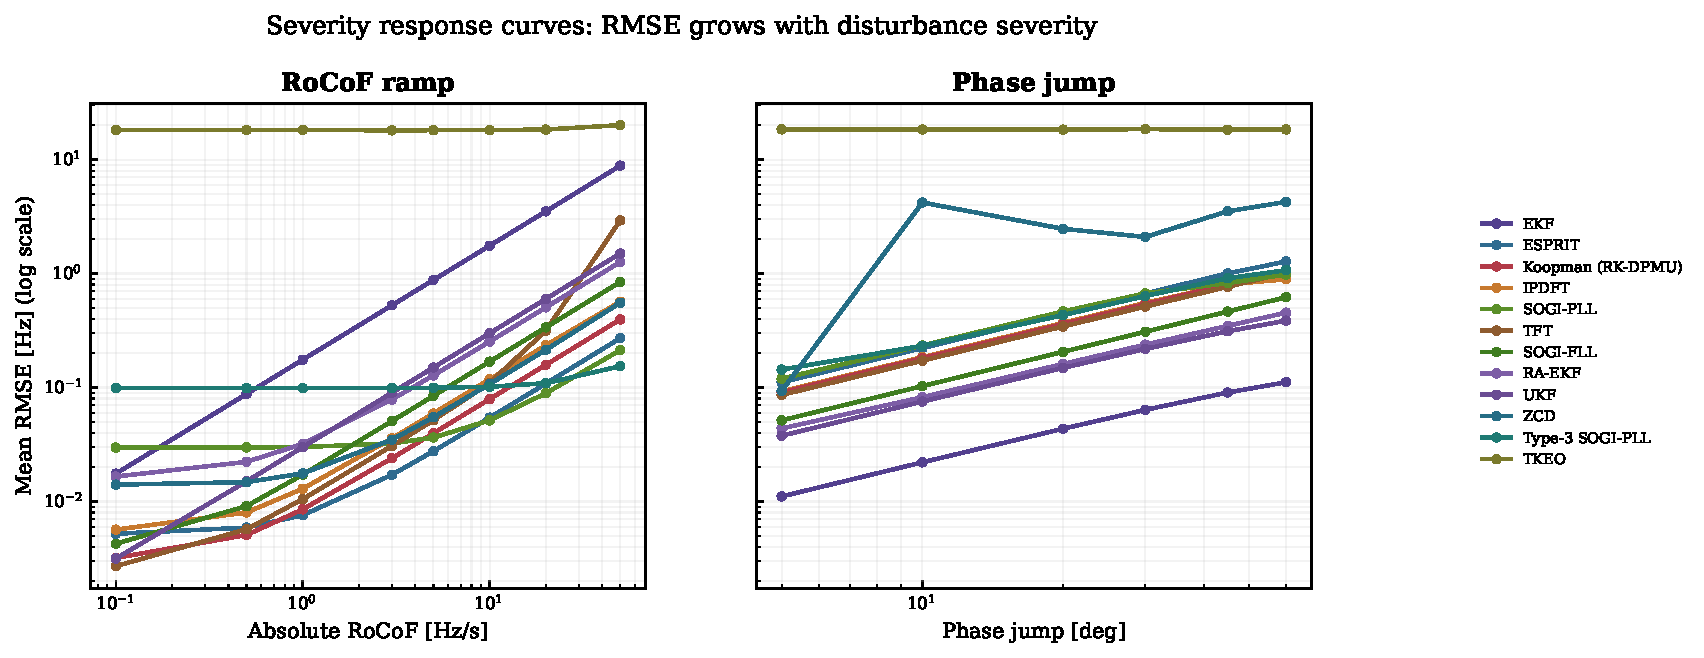
\includegraphics[width=0.97\linewidth,height=0.64\textheight,keepaspectratio]{figures/severity_curves_dynamic.pdf}
\end{frame}

\begin{frame}{Severity response: harmonics and broadband noise}
\papergradebanner
\centering
{\scriptsize\color{ofbMuted}Spectral and noise stress: several methods hold a low-error plateau, then cross a cliff into the unusable regime as severity rises.}
\vspace{0.25em}
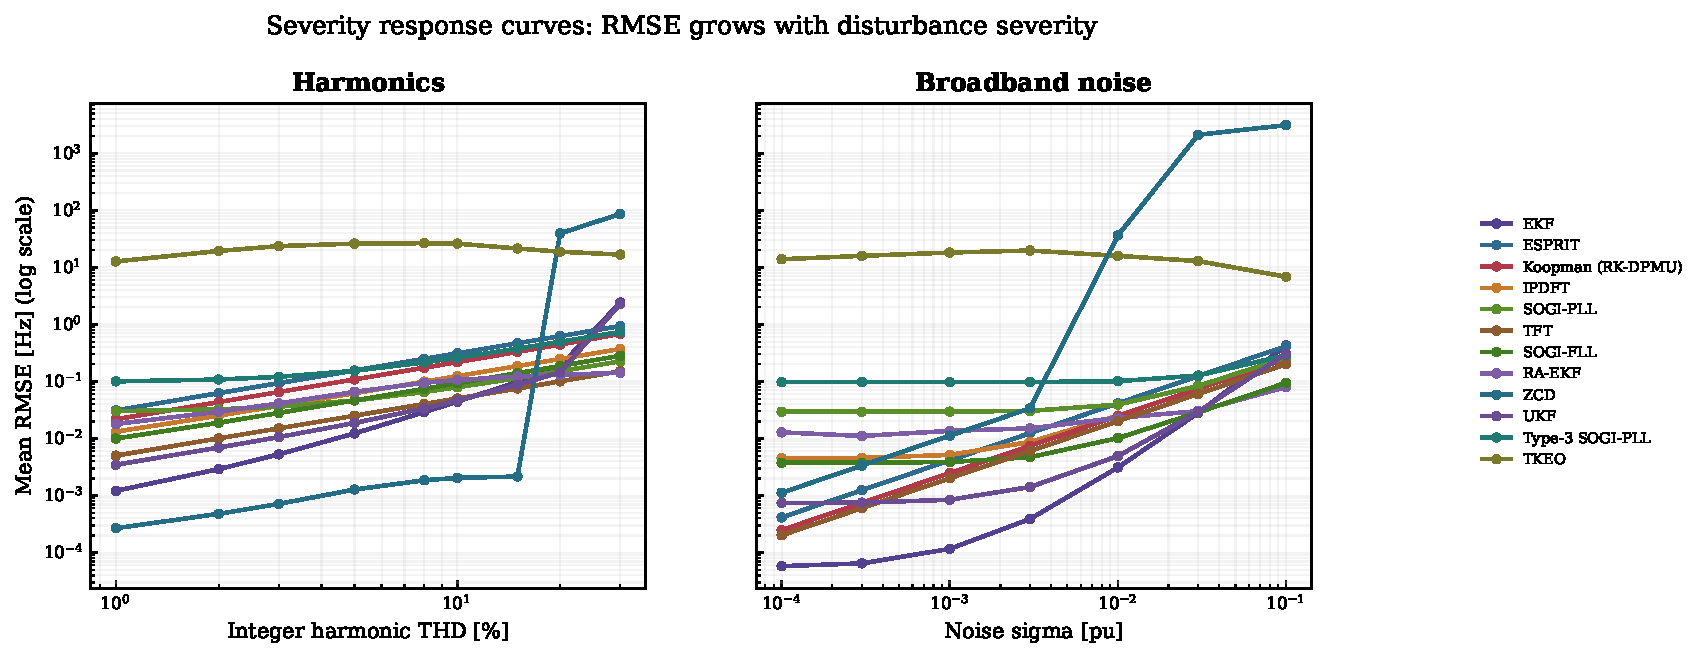
\includegraphics[width=0.97\linewidth,height=0.64\textheight,keepaspectratio]{figures/severity_curves_spectral.pdf}
\end{frame}

\section{Deployment}
\sectionframe{}{Deployment \& Conclusion}{Recommendations and validation agenda}

\begin{frame}[label=recommendationmap]{Recommendation map}
\begin{center}
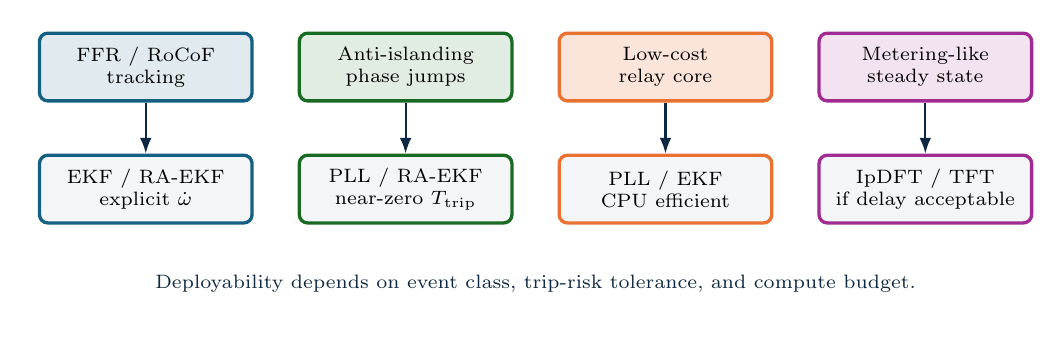
\begin{tikzpicture}[
  every node/.style={font=\scriptsize},
  task/.style={draw, rounded corners=3pt, minimum width=2.7cm, minimum height=0.86cm, align=center, very thick},
  arr/.style={-{Latex[length=2mm]}, thick, color=ofbInk}
]
% fixed canvas so the centred diagram does not re-centre between overlays
\useasboundingbox (-1.5,-1.95) rectangle (11.3,1.7);
\node<1->[task, fill=ofbBlue!13, draw=ofbBlue] (monitor) at (0,1.2) {FFR / RoCoF\\tracking};
\node<2->[task, fill=ofbGreen!13, draw=ofbGreen] (dyn) at (3.3,1.2) {Anti-islanding\\phase jumps};
\node<3->[task, fill=ofbGold!18, draw=ofbGold] (rocof) at (6.6,1.2) {Low-cost\\relay core};
\node<4->[task, fill=ofbViolet!13, draw=ofbViolet] (harm) at (9.9,1.2) {Metering-like\\steady state};
\node<1->[task, fill=ofbSoft, draw=ofbBlue] (m1) at (0,-0.35) {EKF / RA-EKF\\explicit $\dot\omega$};
\node<2->[task, fill=ofbSoft, draw=ofbGreen] (m2) at (3.3,-0.35) {PLL / RA-EKF\\near-zero $T_{\mathrm{trip}}$};
\node<3->[task, fill=ofbSoft, draw=ofbGold] (m3) at (6.6,-0.35) {PLL / EKF\\CPU efficient};
\node<4->[task, fill=ofbSoft, draw=ofbViolet] (m4) at (9.9,-0.35) {IpDFT / TFT\\if delay acceptable};
\draw<1->[arr] (monitor) -- (m1);
\draw<2->[arr] (dyn) -- (m2);
\draw<3->[arr] (rocof) -- (m3);
\draw<4->[arr] (harm) -- (m4);
\node<5->[align=center, text=ofbInk] at (4.95,-1.55) {Deployability depends on event class, trip-risk tolerance, and compute budget.};
\end{tikzpicture}
\end{center}
\end{frame}

\begin{frame}[label=threefindings]{Three findings}
\vspace{0.15em}
\begin{columns}[T,onlytextwidth]
\column{0.32\linewidth}
\insightcard{ofbBlue}{1. Metric-conditioned}{The MC benchmark and ATLAS both show that RMSE, trip exposure, RoCoF, and CPU can select different methods.}
\column{0.32\linewidth}
\insightcard{ofbRust}{2. Stress-bounded}{AM remains survivable for many methods; severe FM, RoCoF, interharmonics, noise, and extreme THD break the 0.05 Hz guide.}
\column{0.32\linewidth}
\insightcard{ofbGreen}{3. Robustness over point accuracy}{Low point error does not imply robustness: RA-EKF stays within band on every ramp seed in the tested run.}
\end{columns}
\vspace{0.5em}
\resultclaim{ofbBlue}{Dynamic frequency estimators should be qualified by event family, sign, severity, recovery, trip exposure, and compute envelope.}
\end{frame}

\begin{frame}[label=validationconclusion]{Conclusion and roadmap}
\begin{columns}[T,onlytextwidth]
\column{0.49\linewidth}
\begin{block}{Conclusion}
\scriptsize
\begin{itemize}
  \item Field disturbances define the measurement problem; controlled synthetic truth makes estimator behavior explainable.
  \item The study compares estimators across objectives, regimes, and deployment constraints, including IBR-relevant stress modes.
  \item Empirical conclusions remain tied to evidence level, stress regime, and replication depth.
\end{itemize}
\end{block}
\column{0.49\linewidth}
\begin{block}{Future work --- roadmap}
\scriptsize
\begin{itemize}
  \item \textbf{Phase 1:} ANDES transient simulation of IEEE IBR standard-method fault scenarios.
  \item \textbf{Phase 2:} Load the simulation CSVs as benchmark truth and replay every estimator.
  \item \textbf{Phase 3:} HIL with FPGA estimator implementations for real-time validation.
\end{itemize}
\end{block}
\end{columns}
\vspace{-0.15cm}
\callout{\textbf{Result:} estimator choice is tied to event class, metric target, and compute envelope; estimator qualification must declare the stress regime, latency limit, and evidence depth.}
\end{frame}

\section{References}

\begin{frame}{Selected references}
\scriptsize
\begin{columns}[T,onlytextwidth]
\column{0.49\linewidth}
\textbf{\color{ofbBlue}Standards, measurement \& methods}
\begin{itemize}\setlength\itemsep{0.18em}
  \item IEEE/IEC 60255-118-1:2018 --- synchrophasor, frequency, and RoCoF measurement and compliance requirements.
  \item H.~Ahmed, S.~Biricik, M.~Benbouzid, ``Linear Kalman Filter-Based Grid Synchronization Technique: An Alternative Implementation,'' IEEE, 2021 \emph{(LKF2)}.
  \item Open synchrophasor infrastructure: OpenPMU, openPDC, FNET/GridEye, and LBNL/PNNL open PMU event datasets.
\end{itemize}
\column{0.49\linewidth}
\textbf{\color{ofbRust}IBR field-event reports}
\begin{itemize}\setlength\itemsep{0.18em}
  \item NERC/WECC Blue Cut Fire (2017) and Canyon 2 Fire (2018) solar-PV interruption reports.
  \item NERC Odessa I/II disturbance reports (2021, 2022).
  \item NERC/WECC 2022 California BESS disturbance report (2023).
  \item Dong et al., Kaua'i 18--20~Hz oscillation analysis (arXiv:2301.05781).
\end{itemize}
\end{columns}
\vspace{0.5em}
\callout{Full reference list, methodology, and artifacts in the submitted paper.}
\end{frame}

{
\usebackgroundtemplate{\includegraphics[width=\paperwidth,height=\paperheight]{\sgsmaDividerBg}}%
\begin{frame}[plain]
\begin{tikzpicture}[remember picture,overlay]
  \node[anchor=center, text=white, align=center, font=\fontsize{32}{38}\selectfont\rmfamily] at ([yshift=0.75cm]current page.center) {Thank you};
  \node[anchor=center, text=white, align=center, font=\large] at ([yshift=-0.55cm]current page.center) {Questions \& discussion welcome};
  \node[anchor=center, text=white, align=center, font=\small] at ([yshift=-1.65cm]current page.center) {Jorge L. Mayorga Taborda \quad$|$\quad Universidad de los Andes \quad$|$\quad SGSMA 2026};
\end{tikzpicture}
\end{frame}
}

\end{document}
